\documentclass{standalone}
\usepackage{tikz, xcolor}
\usetikzlibrary{shapes,arrows}

\begin{document}

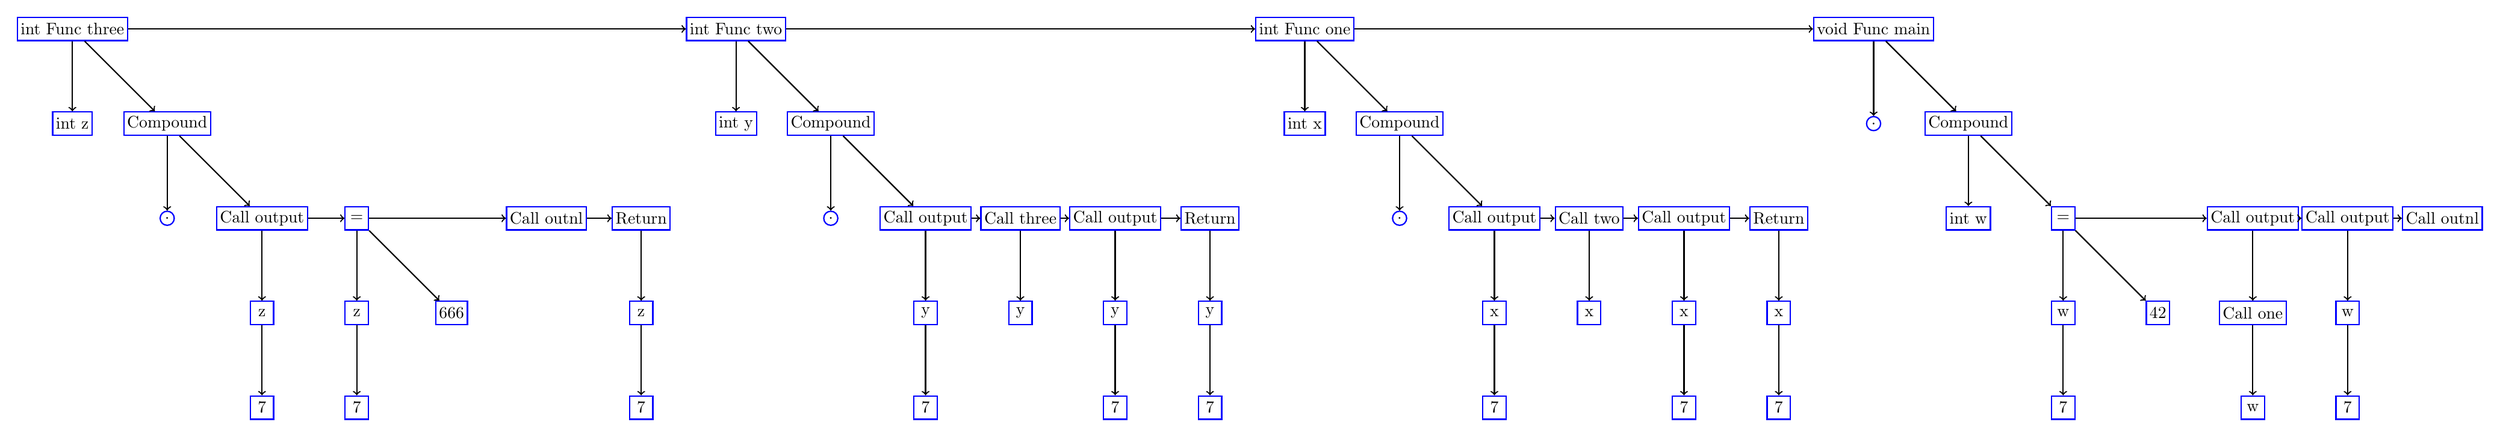
\begin{tikzpicture}[thick, scale=2.0]
\tikzstyle{vertexr}=[rectangle, draw=blue, thick, minimum size=14pt, inner sep=2pt]
\tikzstyle{vertexc}=[circle, draw=blue, thick, inner sep=2pt]
\tikzstyle{drawstyle}=[thick, ->]

\node[vertexr] (G0x0) at (0,0) {int Func three};
\node[vertexr] (G0x1) at (0,-1) {int z};
\draw[drawstyle] (G0x0) -- (G0x1);
\node[vertexr] (G1x1) at (1,-1) {Compound};
\node[vertexc] (G1x2) at (1,-2) {.};
\draw[drawstyle] (G1x1) -- (G1x2);
\node[vertexr] (G2x2) at (2,-2) {Call output};
\node[vertexr] (G2x3) at (2,-3) {z};
\node[vertexr] (G2x4) at (2,-4) {7};
\draw[drawstyle] (G2x3) -- (G2x4);
\draw[drawstyle] (G2x2) -- (G2x3);
\node[vertexr] (G3x2) at (3,-2) {=};
\node[vertexr] (G3x3) at (3,-3) {z};
\node[vertexr] (G3x4) at (3,-4) {7};
\draw[drawstyle] (G3x3) -- (G3x4);
\draw[drawstyle] (G3x2) -- (G3x3);
\node[vertexr] (G4x3) at (4,-3) {666};
\draw[drawstyle] (G3x2) -- (G4x3);
\node[vertexr] (G5x2) at (5,-2) {Call outnl};
\node[vertexr] (G6x2) at (6,-2) {Return};
\node[vertexr] (G6x3) at (6,-3) {z};
\node[vertexr] (G6x4) at (6,-4) {7};
\draw[drawstyle] (G6x3) -- (G6x4);
\draw[drawstyle] (G6x2) -- (G6x3);
\draw[drawstyle] (G5x2) -- (G6x2);
\draw[drawstyle] (G3x2) -- (G5x2);
\draw[drawstyle] (G2x2) -- (G3x2);
\draw[drawstyle] (G1x1) -- (G2x2);
\draw[drawstyle] (G0x0) -- (G1x1);
\node[vertexr] (G7x0) at (7,0) {int Func two};
\node[vertexr] (G7x1) at (7,-1) {int y};
\draw[drawstyle] (G7x0) -- (G7x1);
\node[vertexr] (G8x1) at (8,-1) {Compound};
\node[vertexc] (G8x2) at (8,-2) {.};
\draw[drawstyle] (G8x1) -- (G8x2);
\node[vertexr] (G9x2) at (9,-2) {Call output};
\node[vertexr] (G9x3) at (9,-3) {y};
\node[vertexr] (G9x4) at (9,-4) {7};
\draw[drawstyle] (G9x3) -- (G9x4);
\draw[drawstyle] (G9x2) -- (G9x3);
\node[vertexr] (G10x2) at (10,-2) {Call three};
\node[vertexr] (G10x3) at (10,-3) {y};
\draw[drawstyle] (G10x2) -- (G10x3);
\node[vertexr] (G11x2) at (11,-2) {Call output};
\node[vertexr] (G11x3) at (11,-3) {y};
\node[vertexr] (G11x4) at (11,-4) {7};
\draw[drawstyle] (G11x3) -- (G11x4);
\draw[drawstyle] (G11x2) -- (G11x3);
\node[vertexr] (G12x2) at (12,-2) {Return};
\node[vertexr] (G12x3) at (12,-3) {y};
\node[vertexr] (G12x4) at (12,-4) {7};
\draw[drawstyle] (G12x3) -- (G12x4);
\draw[drawstyle] (G12x2) -- (G12x3);
\draw[drawstyle] (G11x2) -- (G12x2);
\draw[drawstyle] (G10x2) -- (G11x2);
\draw[drawstyle] (G9x2) -- (G10x2);
\draw[drawstyle] (G8x1) -- (G9x2);
\draw[drawstyle] (G7x0) -- (G8x1);
\node[vertexr] (G13x0) at (13,0) {int Func one};
\node[vertexr] (G13x1) at (13,-1) {int x};
\draw[drawstyle] (G13x0) -- (G13x1);
\node[vertexr] (G14x1) at (14,-1) {Compound};
\node[vertexc] (G14x2) at (14,-2) {.};
\draw[drawstyle] (G14x1) -- (G14x2);
\node[vertexr] (G15x2) at (15,-2) {Call output};
\node[vertexr] (G15x3) at (15,-3) {x};
\node[vertexr] (G15x4) at (15,-4) {7};
\draw[drawstyle] (G15x3) -- (G15x4);
\draw[drawstyle] (G15x2) -- (G15x3);
\node[vertexr] (G16x2) at (16,-2) {Call two};
\node[vertexr] (G16x3) at (16,-3) {x};
\draw[drawstyle] (G16x2) -- (G16x3);
\node[vertexr] (G17x2) at (17,-2) {Call output};
\node[vertexr] (G17x3) at (17,-3) {x};
\node[vertexr] (G17x4) at (17,-4) {7};
\draw[drawstyle] (G17x3) -- (G17x4);
\draw[drawstyle] (G17x2) -- (G17x3);
\node[vertexr] (G18x2) at (18,-2) {Return};
\node[vertexr] (G18x3) at (18,-3) {x};
\node[vertexr] (G18x4) at (18,-4) {7};
\draw[drawstyle] (G18x3) -- (G18x4);
\draw[drawstyle] (G18x2) -- (G18x3);
\draw[drawstyle] (G17x2) -- (G18x2);
\draw[drawstyle] (G16x2) -- (G17x2);
\draw[drawstyle] (G15x2) -- (G16x2);
\draw[drawstyle] (G14x1) -- (G15x2);
\draw[drawstyle] (G13x0) -- (G14x1);
\node[vertexr] (G19x0) at (19,0) {void Func main};
\node[vertexc] (G19x1) at (19,-1) {.};
\draw[drawstyle] (G19x0) -- (G19x1);
\node[vertexr] (G20x1) at (20,-1) {Compound};
\node[vertexr] (G20x2) at (20,-2) {int w};
\draw[drawstyle] (G20x1) -- (G20x2);
\node[vertexr] (G21x2) at (21,-2) {=};
\node[vertexr] (G21x3) at (21,-3) {w};
\node[vertexr] (G21x4) at (21,-4) {7};
\draw[drawstyle] (G21x3) -- (G21x4);
\draw[drawstyle] (G21x2) -- (G21x3);
\node[vertexr] (G22x3) at (22,-3) {42};
\draw[drawstyle] (G21x2) -- (G22x3);
\node[vertexr] (G23x2) at (23,-2) {Call output};
\node[vertexr] (G23x3) at (23,-3) {Call one};
\node[vertexr] (G23x4) at (23,-4) {w};
\draw[drawstyle] (G23x3) -- (G23x4);
\draw[drawstyle] (G23x2) -- (G23x3);
\node[vertexr] (G24x2) at (24,-2) {Call output};
\node[vertexr] (G24x3) at (24,-3) {w};
\node[vertexr] (G24x4) at (24,-4) {7};
\draw[drawstyle] (G24x3) -- (G24x4);
\draw[drawstyle] (G24x2) -- (G24x3);
\node[vertexr] (G25x2) at (25,-2) {Call outnl};
\draw[drawstyle] (G24x2) -- (G25x2);
\draw[drawstyle] (G23x2) -- (G24x2);
\draw[drawstyle] (G21x2) -- (G23x2);
\draw[drawstyle] (G20x1) -- (G21x2);
\draw[drawstyle] (G19x0) -- (G20x1);
\draw[drawstyle] (G13x0) -- (G19x0);
\draw[drawstyle] (G7x0) -- (G13x0);
\draw[drawstyle] (G0x0) -- (G7x0);
\end{tikzpicture}
\end{document}
Number of warnings: 0
Number of errors: 0
